\section {Adapters}
\label{ADAPT}

Version 1.2 introduces \emph{Adapters}, a powerful feature that
makes the framework perform some standard and boring activities
autonomously.

\subsection{Introduction}

Previous sections presented the framework and its main feature, that
is -- to recap it once again -- to provide a full support for
separating the logical and the presentation sides of an
application. This separation is featured by the \mvc and the \obs.

Although features are important, \emph{goals} are the driving
targets that lead the framework development. Most important goals of
the framework are to keep simplicity, transparency and lightness,
and to bear the level of abstraction high whilst still allowing to
control and customise lower levels.

It is the case that the framework forces and helps to both design
and implement applications in a clean and robust way. 

However, sometimes things get complicated even for simple
designs. In particular \kw{Controllers} tend to blow up in size and
complexity when handling a \kw{View} containing many widgets, and
when observing many properties into the \kw{Model}. Also, since the
framework can handle several kinds of observable properties (\OPS),
developers are required to remember and to define some naming
conventions for notifications methods defined inside \kw{Observers}
that contributes to make things that would be easy too complex.

In particular, when a default behaviour is expected, the
\kw{Controller} gets filled in with many methods whose code follows
a template that is identically repeated all over again. 

\bigskip 

For example, let us suppose it is needed to have a text entry always
aligned with some part of the model. This would require to have a
textual observable property into the model, a signal handler into
the controller to handle the \codename{'changed'} signal, and a
method to handle notification for observable property value
changes. When a \codename{'changed'} signal arrives, the signal
handle should read the text entry value and report it to the
observable property into the model. Viceversa, when the observable
property in the model get changed for any reason, the notification
code into the controller should update the text entry value. This 
code should also avoid to fall into a reciprocal loop. 

\smallskip
It is in this context that adapters become pretty nifty. 

\subsection{What are Adapters}

\kw{Adapters} are the generalization of the the code that handles
autonomously the connection between a set of widgets and a
corresponding set of properties (possibly observable) to keep
aligned automatically the logical and the presentation sides, and to
keep low the complexity of controllers.

\begin{figure}[htbp]
\begin{center}
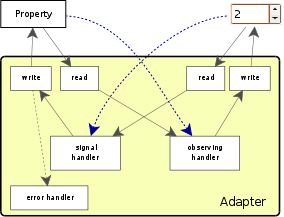
\includegraphics[width=10cm]{figs/png/adap}
\caption{\label{ADAP_f} Schematic simple adapter}
\end{center}
\end{figure}

In figure \ref{ADAP_f} is represented a simple adapter, where main
internal functional blocks are shown. There exist functional blocks
to control the way the property and the widget are read and written,
and how errors are handled when exceptions occur when writing into
the property.

An Adapter \emph{adapts} widgets and model's properties. Adapters
offer strong customization, but in their simplest use their are
pretty easy to be used. in this context, previous example might be
handled as follows.

We have a hand-made View with containing a button and a text
entry. Notice that the name of the text entry is
\codename{entry\_text}.

{ \codesize
\begin{verbatim}
class MyView (gtkmvc.View):
    def __init__(self, ctrl):
        gtkmvc.View.__init__(self, ctrl, register=False)

        w = gtk.Window(); e = gtk.Entry(); b = gtk.Button("Press")

        h = gtk.VBox(); h.add(e); h.add(b); w.add(h)
        w.show_all()
        self['entry_text'] = e
        self['button'] = b
        
        ctrl.register_view(self)
        return
    pass # end of class
\end{verbatim}
}


The model contains simply an observable properties that should
reflect the content of the text entry \codename{entry\_text}.

{ \codesize
\begin{verbatim}
class MyModel (gtkmvc.Model):
    __properties__ = {
        'text' : "Ciao",
        }
    pass # end of class
\end{verbatim}
}

As usual, the controller is the most complex part, but by exploiting
an adapter it gets pretty much simplified. 
{ \codesize
\begin{verbatim}
class MyCtrl (gtkmvc.Controller):
    def register_adapters(self):
        self.adapt("text")
        return

    def register_view(self, view):
        gtkmvc.Controller.register_view(self, view)
        view['button'].connect('clicked', self.on_button_clicked)
        return

    # signal handles
    def on_button_clicked(self, button):
        print "Text is:'%s'" % self.model.text
        return

    pass # end of class
\end{verbatim}
}

The idea of this example is to have ``\codename{button}''
that when pressed makes model's observable property \codename{text}
printed out to the standard output.

No code is included to handle \codename{entry\_text} ``change''
signal and observable property value change notifications. Instead,
a new method surfaces off the controller:
\codename{register\_adapters}.

This method is called at the right time by the framework and it is a
good place where adapters can be created and connected. In the
example, creation occurs through a call to another new method of
class Controller: \codename{adapt}. 

The new method is pretty complex and will be discussed in depth
later. Enough to say now is that parameter \codename{"text"}
represents the name of the observable property that we want to
adapt. The corresponding widget is searched among all widgets in the
view, and widget \codename{entry\_text} is found and connected
automatically. The way this magic happens is not important at this
stage, but soon you will introduced with all details, to make you
know how to fully exploit and control this new feature.

\begin{figure}[htbp]
\begin{center}
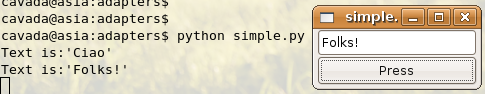
\includegraphics[width=10cm]{figs/png/adap1}
\caption{\label{ADAP1_f} Simple adapter at work}
\end{center}
\end{figure}


The code that instantiates and runs this example is as usual:
{ \codesize
\begin{verbatim}
m = MyModel()
c = MyCtrl(m)
v = MyView(c)
gtk.main()
\end{verbatim}
}

File \file{examples/adapters/simple.py} contains the full source
code of this example. When being run, it shows up a window
containing the text entry and the button. When the button is
pressed, the content of the observable property \codename{text} is
printed to the standard output. Initially, \codename{text} is
assigned to \codename{"Ciao"} and the text entry reflects it
accordingly.

If the user changes the text in the entry, the property
\codename{text} will be changed accordingly, as it is easy to check
by clicking the button.


\subsection{Module \codename{adapters}}
Currently, module \codename{adapters} contains a few adapters types.

\begin{description}
\item [\codename{Adapter}] Connects a widget and a property. The
  property cannot be a container or a user-defined class.

\item [\codename{UserClassAdapter}] This class handles the
  communication between a widget and a class instance that is a
  property inside the model.

\item [\codename{RoUserClassAdapter}] This is similar to
  \codename{UserClassAdapter}, but dedicated to read-only class
  instances. Used internally to handle for example
  \codename{datetime} properties, when connecting a
  \codename{gtk.Calendar}.

\item [\codename{StaticContainerAdapter}] This class can be used to
  bound a set of widgets to a single property that is a container,
  like a tuple, a list or a map, or in general a class that
  implements \codename{\_\_getitem\_\_} and
  \codename{\_\_setitem\_\_} methods.
\end{description}


\subsubsection{Class \codename{Adapter}}
This is the base class for all adapters. All adapters derive from
class \codename{Observer}. Instantiation of an Adapter can be
optionally complex and customizable by using same optional
parameters. Available parameters are presented here, but examples
will show them applied in a practical manner. 

Important operations are:

\begin{description}
\item [Constructor] Class constructor gets several parameters, but
  only two are strictly required.
{
\codesize
\begin{verbatim}
def __init__(self, model, prop_name, 
             prop_read=None, prop_write=None, 
             value_error=None)
\end{verbatim}
}

\begin{description}
  \item [\codename{model}] is the Model instance containing the
    property to be observed.

  \item [\codename{prop\_name}] is the model's property name (as a
    string). It is possible to use a dotted notation to identify a
    property contained into a hierarchy of models. For example
    'a.b.c' identifies property 'c' into model 'b' inside model 'a',
    where model 'a' is an attribute of given top level model. Last
    name can be an observable or non-observable attribute, and
    previous names (if specified) must all refer to instances of
    class \codename{Model}. First name from the left must be the
    name of a model instance inside the given model.

  \item [\codename{prop\_read}] optional function that apply custom
    modifications to the value of the property before reading
    it. The function takes a value and must return a transformed
    value. Use to customize the way the property is read, and to
    apply useful transformations to the read value.

  \item [\codename{prop\_write}] Like \codename{prop\_read} optional
    function that apply custom modifications to the value of the
    property before writing it. The function takes a value and must
    return a transformed value whose type must be compatible with
    the type of the property. Use to customize the way the property
    is written, and to apply useful transformations to the value.

  \item [\codename{value\_error}] optional parameter that can be a
    function (or a method) to be called when a \codename{ValueError}
    exception occurs while trying to set a wrong value for the
    property inside the model. The function will receive: the
    adapter, the property name and the value coming from the widget
    that offended the model. Useful to catch and handle error
    conditions.

\end{description}

\item [Widget connection] Constructor connects properties, while
  widgets are connected through method \codename{connect\_widget}:

{
\codesize
\begin{verbatim}
def connect_widget(self, widget,
                   getter=None, setter=None, 
                   signal=None, arg=None, update=True)
\end{verbatim}
}

\begin{description}

\item [widget] is the widget that is needed to connect
\item[getter] optional function used to ``read'' the
  widget. The function receives a widget instance.
\item[setter] optional function used to ``write'' the
  widget. The function receives a widget instance and the value to
  be written.
\item[signal] Optional name of the signal that will be used to
  monitor the widget changes.
\item[arg] Optional argument that is passed to the signal
  handler. It will be used when connecting the signal.
\item[update] If False, the widget will be not initially updated
  with the initial value of the property. Used in very particular
  conditions.
\end{description}

\item[update\_model()] Forces the property to be updated from the
  value hold by the widget. This method should be called directly by
  the user in very unusual conditions.

\item[update\_widget()] Forces the widget to be updated from the
  property value. This method should be called directly by the user
  when the property is not observable, or in very unusual conditions.

\end{description}


At this step thorough people would be asking them self how
instantiation of adapters can work in its simplest option, i.e. by
specifying the minimal set of parameters, and exploiting all default
values for the others.

The framework searches information about widgets and possible
default values for any unspecified parameter into module
\file{adapters.default}.

Suppose for example that the specified widget is a
\codename{gtk.Entry}. Good candidates for unspecified
\codename{getter} and \codename{setter} would be
\codename{gtk.Entry.get\_text} and \codename{gtk.Entry.set\_text}
respectively. \codename{signal} will be \codename{"changed"} to
capture events that change the value of the widget.

Later a list of all currently supported widgets will be presented.


\subsubsection{Class \codename{UserClassAdapter}}

This class handles the communication between a widget and a class
instance (possibly observable) that is a property inside the
model. The value to be shown is taken and stored by using a getter
and a setter. getter and setter can be: names of user class methods,
bound or unbound methods of the user class, or a function that will
receive the user class instance and possible arguments whose number
depends on whether it is a getter or a setter.

Class \codename{UserClassAdapter} derives directly from class
\codename{Adapter} and redefines the constructor as follow.

{
\codesize
\begin{verbatim}
  def __init__(self, model, prop_name,
               getter, setter, 
               prop_read=None, prop_write=None,                   
               value_error=None):
\end{verbatim}
}

Where \codename{getter} and \codename{setter} are two new required
parameters, and all the other are unchanged.

\begin{description}
\item [\codename{getter}] can be a string holding the name of the
  user class method, a bound or unbound method of the user class, or
  a function that will receive the user class instance. The function
  or method is required to return the value to be read into the user
  class.

\item [\codename{setter}] can be a string holding the name of the
  user class method, a bound or unbound method of the user class, or
  a function that will receive the user class instance and a value
  for setting. 
\end{description}



\subsubsection{Class \codename{StaticContainerAdapter}}
This class can be used to bound a set of widgets to a property that
is a container, like a tuple, a list or a map, or in general a class
that implements \codename{\_\_getitem\_\_} and
\codename{\_\_setitem\_\_} methods.

From the other hand, the set of widgets can be a list provided by
the user, or a container widget like a Box, a Notebook, etc.
Widgets will be linked by their position when the property is
list-like, or by their names or instances when the property is
map-like.

This class supports only properties that are static containers,
i.e. those containers that do not change their length
dynamically. If the container grows up in length, no change will
occur in the view-side.

This class derives from class \codename{UserClassAdapter}.

\begin{description}

\item [Widget connection] Different than Adapter's method,
  \codename{connect\_widget} accepts sets.

{ 
\codesize
\begin{verbatim}
def connect_widget(self, widget,
                   getters=None, setters=None, 
                   signals=None, arg=None)
\end{verbatim}
}

\begin{description}

\item [widget] is either a container widget, or a list of widgets. 
\item[getters] optional function or list or a map of functions used
  to ``read'' the widget(s). Each function receives a widget
  instance.
\item[setters] optional function or list or a map of functions used
  to ``write'' the widget(s). Each function receives a widget
  instance and value for setting.

\item[signal] can be None, a signal name, or a list or a map of
  signal names.

\item[arg] Optional argument that is passed to each signal
  handler. It will be used when connecting the signal(s). 
\end{description}

When maps are used, keys can be widgets or widget names. The length
of the possible lists or maps must be lesser or equal to the number
of widgets that will be connected.

\item[update\_model(idx=None)] Updates the value of property at
  given index. If \codename{idx} is \codename{None}, all controlled
  indices will be updated. This method should be called directly by
  the user in very unusual conditions.

\item[update\_widget(idx=None)] Forces the widget at given index to
  be updated from the property value. If index is not given, all
  controlled widgets will be updated. This method should be called
  directly by the user when the property is not observable, or in
  very unusual conditions.
\end{description}

Since things got a bit convoluted here, some examples can help to
understand how this kind of adapter can be used. 


Suppose you have a glade file containing a button and a
\codename{HBox} called \codename{"hbox"} containing a text entry, a
label and a \codename{SpinButton}.

\begin{figure}[here]
\begin{center}
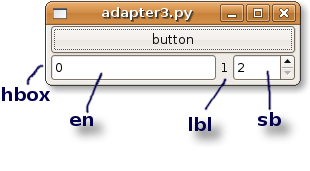
\includegraphics[width=4cm]{figs/png/adap2}
\caption{\label{ADAP2_f} \codename{StaticContainerAdapter} at work}
\end{center}
\end{figure}

The view is simply:

{ \codesize
  \begin{verbatim}
class MyView (View):
    def __init__(self, ctrl):
        View.__init__(self, ctrl, "adapters.glade", "window")
        return
    pass # end of class
  \end{verbatim}
}

The model contains a tuple of three integers that we want to connect
to the widgets into the \codename{HBox}. When the button is clicked,
one of the three integers is randomly incremented.

{ \codesize
  \begin{verbatim}
class MyModel (Model):
    __properties__ = {
       'box' : [0,1,2]
       }
    pass # end of class
  \end{verbatim}
}

The controller handles the button click signal:
{ \codesize
  \begin{verbatim}
import random
class MyCtrl (Controller):
    def on_button_clicked(self, button):
        self.model.box[random.randint(0,2)] += 1
        return
    pass # end of class
  \end{verbatim}
}

If typically construction of adapters occurs into method
\codename{register\_adapters} for the sake of simplicity in this
example instantiation of the adapter is located in the main
launching code:

{ \codesize
\begin{verbatim}
m = MyModel()
c = MyCtrl(m)
v = MyView(c)

a = StaticContainerAdapter(m, "box")
a.connect_widget(v["hbox"])

gtk.main()
\end{verbatim}
}

Adaption of widgets occur by their position into the
\codename{"hbox"} container. 

Second example makes use of an explicit list of widgets, and
exploits also parameter \codename{setters} to customize the way the
label \codename{"lbl"} shows its value.

{ \codesize
\begin{verbatim}
m = MyModel()
c = MyCtrl(m)
v = MyView(c)

a1 = StaticContainerAdapter(m, "box")
a1.connect_widget(map(lambda x: v[x], "en lbl sb".split()), 
                  setters = {'lbl': lambda w, v: 
                     w.set_markup("<big>Val: <b>%d</b></big>" % v)})

gtk.main()
\end{verbatim}
}

\begin{figure}[here]
\begin{center}
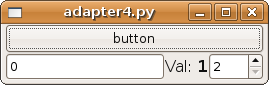
\includegraphics[width=4cm]{figs/png/adap3}
\caption{\label{ADAP3_f} Customized setter for the label}
\end{center}
\end{figure}


Finally, instead of being a tuple, the observable property can be
also a map, whose keys are widget names.

{ \codesize
\begin{verbatim}
class MyModel (Model):
    __properties__ = {
        'box' : { 'en'  : 0,
                  'lbl' : 1,
                  'sb'  : 2 }
        }
    pass # end of class
\end{verbatim}
}

in this case bounding between widgets and values into the property
in the model is carried out by looking at names, and not position.


\subsection{Support for adapter instantiation}
As already seen, since version 1.2 class \codename{Controller}
offers two new methods to support instantiation of adapters. 

\begin{description} 
\item [register\_adapters()] This method is called by the framework
  when it is the best time to create all adapters. All that users
  are required to do is to override this method into their
  controllers derived from \codename{Controller}.

\item [adapt(...)] This method can be used within
  \codename{register\_adapters} to adapt properties and
  widgets. Arguments can be one of the following:

  \begin{enumerate}
  \item Property name as a string. A corresponding widget is
    searched among view's widgets and if only one match is found, a
    default adapter is created. The type of the created adapter
    depends both on the property and the widget type. Widget name
    matching is performed by searching the property name into widget
    names, case insensitive.

  \item Property name and widget name. Like previous but widget name
    is explicitly declared.

  \item An instance of an Adapter. The adapter must be already
    connected to a widget.
  \end{enumerate}

  The first two flavors of method \codename{adapt} allows for an
  easy construction of a default adapter, but only the third allows
  for a full control.

\end{description}


\subsection{Supported widgets}
\label{SUPW}

Here follows the list of those widgets that are currently supported
by the framework out of the box. In method
\codename{Controller.adapt} when adapting a widget, it is searched
into this list a matching and one or more adapters are created.

If no matching is found, a fallback tentative is to connect to
widget signal \codename{"changed"} if there exists. If this fails,
an assertion is raised.

If a widget is not listed here, it does not mean that it is not
supported. Instead, it will be enough to specify all required
parameters when instantiating adapters.

\begin{center}
\begin{tabular}{|l|l|l|}
\hline
Widget type & Property type & Notes\\[0.5ex]
\hline
\codename{gtk.Arrow} & \codename{gtk.ArrowType} & Current direction\\
\codename{gtk.Calendar} & \codename{datetime} or \codename{date} & Selected day\\
\codename{gtk.CheckMenuItem} &  \codename{types.BooleanType} & Current toggle state\\
\codename{gtk.ColorButton} & \codename{gtk.gdk.Color}  & Selected colour \\
\codename{gtk.ColorSelection} & \codename{gtk.gdk.Color} & Selected colour\\
\codename{gtk.Entry} & String & Current entry content \\
\codename{gtk.Expander} &  \codename{types.BooleanType} & True if expanded\\
\codename{gtk.Label} & String or number & Label content \\
\codename{gtk.ToggleButton} &  \codename{types.BooleanType} & Current toggle state \\
\hline
\end{tabular} 
\end{center}


